\documentclass{article}
\usepackage{graphicx}
\usepackage{amssymb}
\usepackage{amsmath}
\usepackage{float}
\usepackage{hyperref}


\begin{document}

\title{Robotics 811 - HW 2}
\author{Xiang Zhi Tan}

\maketitle

\section{Q1}
\begin{equation*}
\begin{aligned}
P_2(x) &= f[x_0] + f[x_0, x_1](x - x_0) + f[x_0, x_1,x_2](x-x_0)(x-x_1)\\
&= f[x_0] + f[x_0, x_1]x - f[x_0, x_1]x_0 + f[x_0, x_1,x_2](x^{2} - xx_0 - xx_1 + x_0x_1)\\
P'_2(x) &= f[x_0, x_1] + f[x_0, x_1,x_2](2x - x_0 - x_1)
\end{aligned}
\end{equation*}
where:
\begin{equation*}
\begin{aligned}
f[x_0, x_1] &= \frac{f(x_0) - f(x_1)}{x_0 - x_1} \\
f[x_0, x_1,x_2] & = \frac{\frac{f(x_0) - f(x_1)}{x_0 - x_1} - \frac{f(x_1) - f(x_2)}{x_1 - x_2}}{x_0 - x_2}
\end{aligned}
\end{equation*}
Now,we insert the point at $i = 1$ into $P'_2(x)$
\begin{equation*}
\begin{aligned}
P'_2(\frac{x_0+x_1}{2}) &= f[x_0,x_1] +  f[x_0, x_1,x_2](2 \times \frac{x_0+x_1}{2} - x_0 - x_1)\\
& = f[x_0,x_1] +  f[x_0, x_1,x_2] \times 0\\
& = f[x_0,x_1]
\end{aligned}
\end{equation*}
This proves $P'_2(x)$ at $i = 1$ is equal to $f[x_0,x_1]$.\\
Now,we insert the point at $i = 2$ into $P'_2(x)$
\begin{equation*}
\begin{aligned}
P'_2(\frac{x_1+x_2}{2}) &= f[x_0,x_1] +  f[x_0, x_1,x_2](2 \times \frac{x_1+x_2}{2} - x_0 - x_1)\\
& = \frac{f(x_0) - f(x_1)}{x_0 - x_1} + \frac{\frac{f(x_0) - f(x_1)}{x_0 - x_1} - \frac{f(x_1) - f(x_2)}{x_1 - x_2}}{x_0 - x_2} (x_0 - x_2) \times -1\\
& = \frac{f(x_0) - f(x_1)}{x_0 - x_1} - \frac{f(x_0) - f(x_1)}{x_0 - x_1} + \frac{f(x_1) - f(x_2)}{x_1 - x_2} \\
& = \frac{f(x_1) - f(x_2)}{x_1 - x_2} \\
& = f[x_1,x_2]
\end{aligned}
\end{equation*}
This proves $P'_2(x)$ at $i = 2$ is equal to $f[x_1,x_2]$.\\
\section{Q2}
\subsection*{a}
Firstly, we calculate the values of $f(x_0),....f(x_i)$ which gives us the vector $0, 0.0434,
0.1269, 0.2217, 0.3187, 0.4145, 0.5075$. By plugging it in into the method with the following variables.
$dividedDifferences(6,2.25,xs,fxs)$. The method will return the result:$0.1737$ 
which is equal to the answer given by matlab which is $0.1737$.
\subsection*{b}
\begin{itemize}
	\item Using the procedure at $x=0.05$ with $n=2$, gave the estimate of $4.9878$.
	\item Using the procedure at $x=0.05$ with $n=4$, gave the estimate of $4.9442$
	\item Using the procedure at $x=0.05$ with $n=40$, gave the estimate of $4.5872$
\end{itemize}
The actual value of $f(0.05)$ is $4.5872$ which is same as the estimate of $4.5872$ by $n=40$
\subsection*{2(c)}
The Error estimate is as following:\\
\begin{tabular}{|c|c|}
\hline
$n$ & $E_n$ \\ \hline
2 & 3.4911\\
4 & 2.3584\\
6 & 3.5367\\
8 & 6.4873\\
10 & 12.9702\\
12 & 27.1445\\
14 & 58.4298\\
16 & 128.1824\\
18 & 285.0742\\
20 & 640.9705\\
40 & 2830400\\
\hline
\end{tabular}\\
The Error make sense, because we are trying to fit a polynomial on a non-polynomial function. As the interpolating polynomial will never become the function that we are trying to interpolating and it will only continue to over fitting the function causing massive error at the end of the functions
\section{Q3}
Firstly, we assume the table contains the values $f(X_i),i = 0,...n$ with $n=\frac{1}{n}$ and $x_i = -\frac{\pi}{2} + i\times h$.  If $\bar{x} \in [x_{i-1}, x_i]$ then we are approximating the function with a polynomial of degree 2, $p_1(x)$. From the notes, we know the error must be:
\begin{equation*}
e_1(\bar{x}) = \frac{f'(xi)}{2!}(\bar{x} - x_{i-1})(\bar{x} - x_i)
\end{equation*}
The error of the first term $f'''(x)$ must be 1 as the function is a simple cos function. The error of the second term is estimated as following:
\begin{equation*}
|(\bar{x} - x_{i-1})(\bar{x} - x_i)| \leq \max_{y \in [-h, 0]}|(y-h)y|
\end{equation*}
Let us consider the function $g(y) = (y-h)y = y^2 - yh$. To find the maximum on the interval, we find the derivative of the function, $g'(y) = 2y - h$ and set it to zero $g'(y) = 0$. This means $g'(y) = 0$ if and only if $y = \frac{h}/2$. By inserting the value into the g(y), we find the maximum of $g(y)$. Which is:
\begin{equation*}
\begin{aligned}
g(\frac{h}{2}) &= {\frac{h}{2}}^2 - h(\frac{h}{2})\\
	&= -\frac{h^2}{4}
\end{aligned}
\end{equation*}
Therefore the error for a linear interpolation is:
\begin{equation*}
\begin{aligned}
|e_1(\bar{x})| &\leq \frac{1}{2!} \times 1 \times \frac{h^2}{4}\\
&= \frac{h^2}{8}
\end{aligned}
\end{equation*}
To get the 6 place accuracy, h need to be choose as following:
\begin{equation*}
\begin{aligned}
\frac{h^2}{8} &\leq 5 \times 10^-6\\
	h &= 0.002	
\end{aligned}
\end{equation*}
Therefore, the number of table entries for a linear interpolation is as following:
\begin{equation*}
\begin{aligned}
\frac{\frac{pi}{2} + \frac{3\pi}{2}}{0.002} + 1 \approx 3143
\end{aligned}
\end{equation*}
If we are using a quadratic interpolation, the interval for $\bar{x}$ will be $[x_{i-1}, x_{i+1}]$ instead. The maximum of the error of $(\bar{x} - x_{i-1})(\bar{x} - x_i)(\bar{x} - x_{i+1})$ can be find in the notes, which is $\frac{2}{3}\frac{1}{\sqrt{3}}h^3$. The Error term for the quadratic equation is as following:
\begin{equation*}
\begin{aligned}
|e_2(\bar{x})| &\leq \frac{1}{3!} \times 1 \times \frac{2}{3}\frac{h^3}{\sqrt{3}} \\
&= \frac{h^3}{9\sqrt{3}}
\end{aligned}
\end{equation*}
To get the 6 place accuracy, h need to be choose as following:
\begin{equation*}
\begin{aligned}
\frac{h^3}{9\sqrt{3}} &\leq 5 \times 10^-6\\
	h &\approx 0.019827	
\end{aligned}
\end{equation*}
Therefore, the number of table entries for a linear interpolation is as following:
\begin{equation*}
\begin{aligned}
\frac{\frac{pi}{2} + \frac{3\pi}{2}}{0.019827} + 1 \approx 318
\end{aligned}
\end{equation*}
\section{Q4}
First we observe the graph of the function $x - tan(x) = 0$ around the 200 point to find good values to be tested. 
\begin{figure}[h]
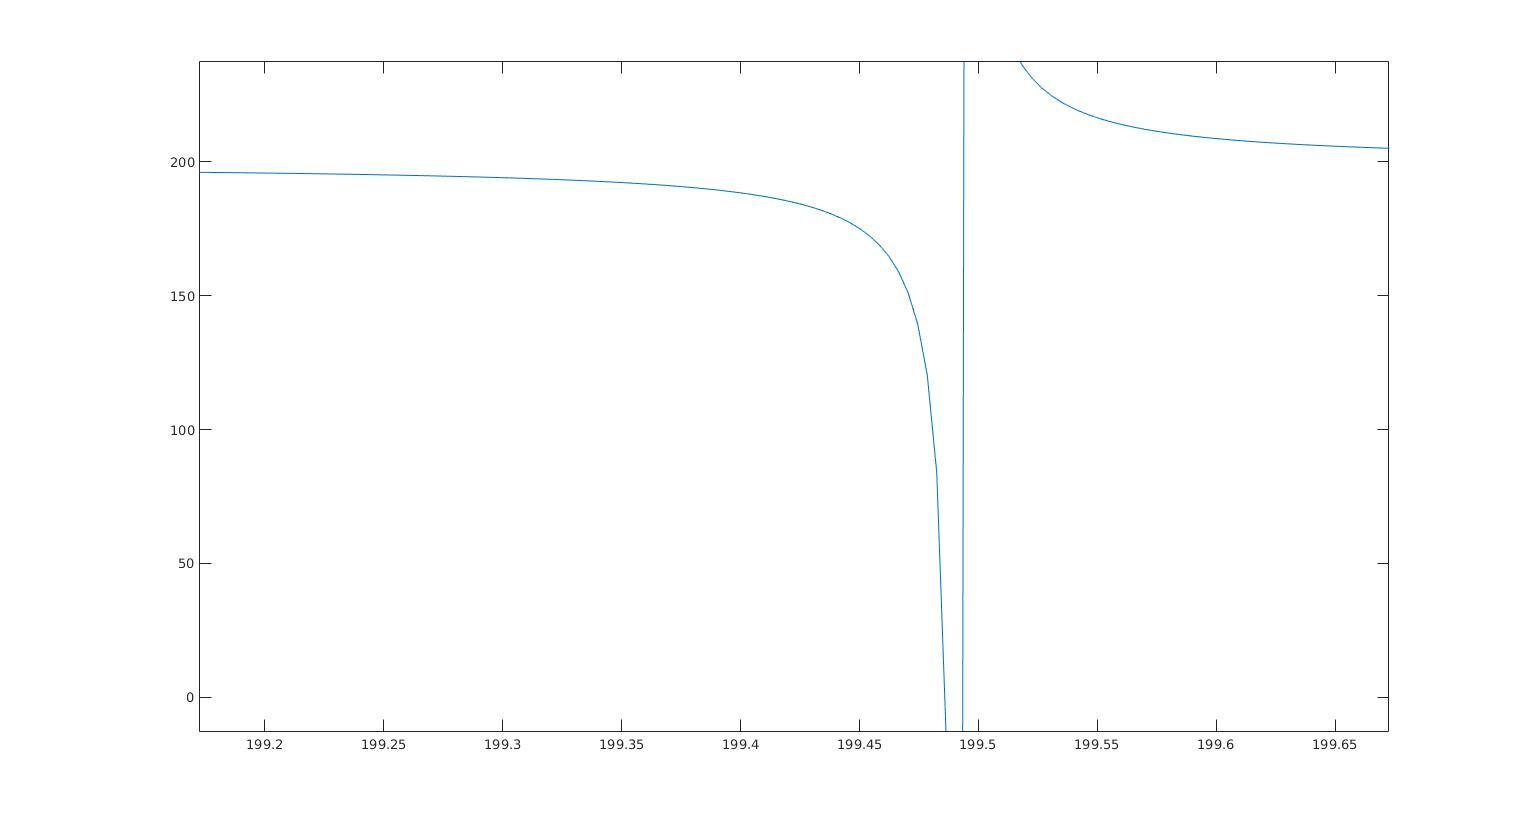
\includegraphics[width=4in]{p4.jpg}
\end{figure}\\
By visual inspection, we found that the root must be between $199.49$ and $199$. We tested this by inserting both values into the function and it gave us both $-682.7305$ and $197.1303$. Since $199.49$ won't be able to converge using Newton Method(implemented in the file titled \textit{newtonMethod.m}), we first use those two values in the bisection method to give an estimate root. The code for the function is attached to this paper under the title \textit{bisectionMethod.m}. The bisectionMethod returns $199.4861$ as the root. As we plugged in the value into newton method, it gave us the same value of $199.4861$. Therefore, the closet root to 200 is $199.4861$
\section{Q5}
\section{Q6}
\subsection{6(a)}
The Muller Method was implemented based on the notes and algorithm given on the website: http://www.physics.arizona.edu/~restrepo/475A/Notes/sourcea-/node25.html . The implementation of the algorithm can be found in the file titled \textit{mullerMethod.m} attached to the homework.
\subsection{6(b)}
first route:
x0 = 4;
x1 = 4.35;
x2 = 4.5;
Root at: 4.4934
second root:
\subsection{6(c)}
We wrote a script called \textit{p6c.m} that runs the algorithm to find the correct k and real roots. First, we visually inspected the graph of the Bessel function at K = 100. This allow us to determine the ranges for the possible roots. Then, we set the initial k to be 3 and loop through the Muller function and slowly increasing k until the root become stable(they did not change since the last iteration). We found the roots to be stable at $k = 31$. The following is the roots found by the algorithm\\
\begin{tabular}{|c|c|c|c|}
\hline
$x_0$ & $x_1$ & $x_2$ & roots \\ \hline
$3$ & $4$ & $5$ & $3.3817$ \\ \hline
$5$ & $6$ & $7$ & $7.0156$ \\ \hline
$9$ & $10$ & $11$ & $10.1735$ \\ \hline
$12$ & $13$ & $14$ & $13.3237$ \\ \hline

\end{tabular}

\section{Q7}
\subsection*{7(a)}
From the two polynomials given, we can construct a Sylvester's matrix:
\begin{equation*}
M = 
\begin{pmatrix}
1 &-12 &41 &-42& 0\\
0 &1   &-23 & 41 & -42\\
1& -2& -35& 0& 0\\
0& 0& 1& -2& -35\\ 
\end{pmatrix}
\end{equation*}
Calculating the determinant will give us
\begin{equation*}
det(M) = -7.1623e-12 \approx 0
\end{equation*}
Because the determinant is approximately 0, this means that $p(x)$ and $q(x)$ shares a common root.
\subsection{7(b)}
Using the ratio method discussed in class we constructed the following equation:
\begin{equation*}
\begin{aligned}
x &= \frac{x^4}{x^3} \\
&=(-1)^{1+2}\frac{det(M_1)}{det(M_2)} \\
&=(-1)\frac{
	\begin{vmatrix}
	-12 & 41 &-42 &  0\\
	  1 &-12 & 41 &-42\\
	 -2 &-35 &  0 &  0\\
	  1 & -2 &-35 &  0\\
	\end{vmatrix}
}{
	\begin{vmatrix}
	  1 & 41 &-42 &  0\\
	  0 &-12 & 41 &-42\\
	  1 &-35 &  0 &  0\\
	  0 & -2 &-35 &  0\\	
	\end{vmatrix}
}\\
&=(-1)\frac{806736}{-115248}\\
&=7
\end{aligned}
\end{equation*}
\section{Q8}
\subsection{8(a)}
The following is the graphing of the following two functions using matlab
\begin{equation*}
\begin{aligned}
p(x,y) &= 2x^2 +2y^2 -1\\
q(x,y) &= x^2 + y^2 + 2xy + x - y
\end{aligned}
\end{equation*}
\begin{figure}[H]
\centering
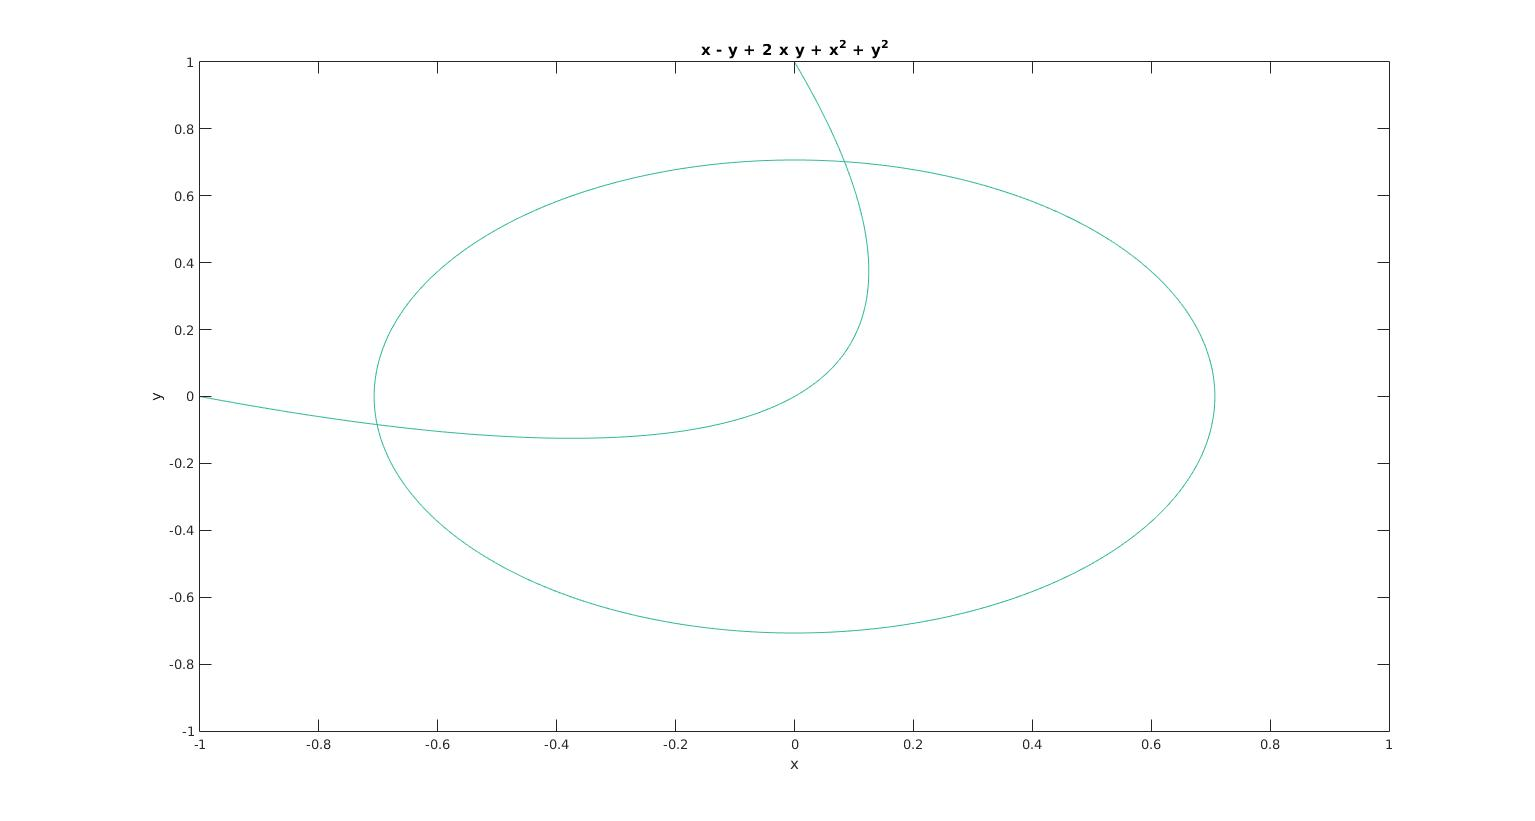
\includegraphics[width=5in]{p8-1.jpg}
\caption{graphing of the two functions}
\end{figure}
\subsection{8(b)}
To find the roots of the equations, we first construct the resultant by eliminating y. The functions are re-written with x as constants.
\begin{equation*}
\begin{aligned}
p(y) &= 2y^2 + (2x^2-1)\\
q(y) &= y^2 + y(2x-1) + (x^2 +x)
\end{aligned}
\end{equation*}
This then could be use to construct the Q matrix
\begin{equation*}
Q = 
\begin{pmatrix}
2 & 0 & 2x^2-1 & 0\\
0 & 2 & 0 & 2x^2 -1 \\
1 & 2x-1 & x^2+x & 0 \\
0 & 1 & 2x-1 & x^2+x\\ 
\end{pmatrix}
\end{equation*}
Using the symbolic toolkit inside matlab, we could determine the determinant of the matrix, $det(Q) = 16x^4 - 16x^3 + 12x - 1$. Using the build in solver in matlab, we were able to solve the 4th degree polynomial, and it gave us 4 different roots (2 real roots and 2 imaginary roots).
\begin{equation*}
\begin{aligned}
   &0.8090 + 0.6360i\\
   &0.8090 - 0.6360i\\
  &-0.7021 \\
   &0.0841 
\end{aligned}
\end{equation*}
We plugged in the two real root into the original algorithm and it gave us the following values
\begin{equation*}
\begin{aligned}
	x: -0.7021 \;&y:0.0840\\
	x: 0.0840 \;&y:0.7021
\end{aligned}
\end{equation*}
\subsection{8(c)}
The result of the roots marked on the graph
\begin{figure}[H]
\centering
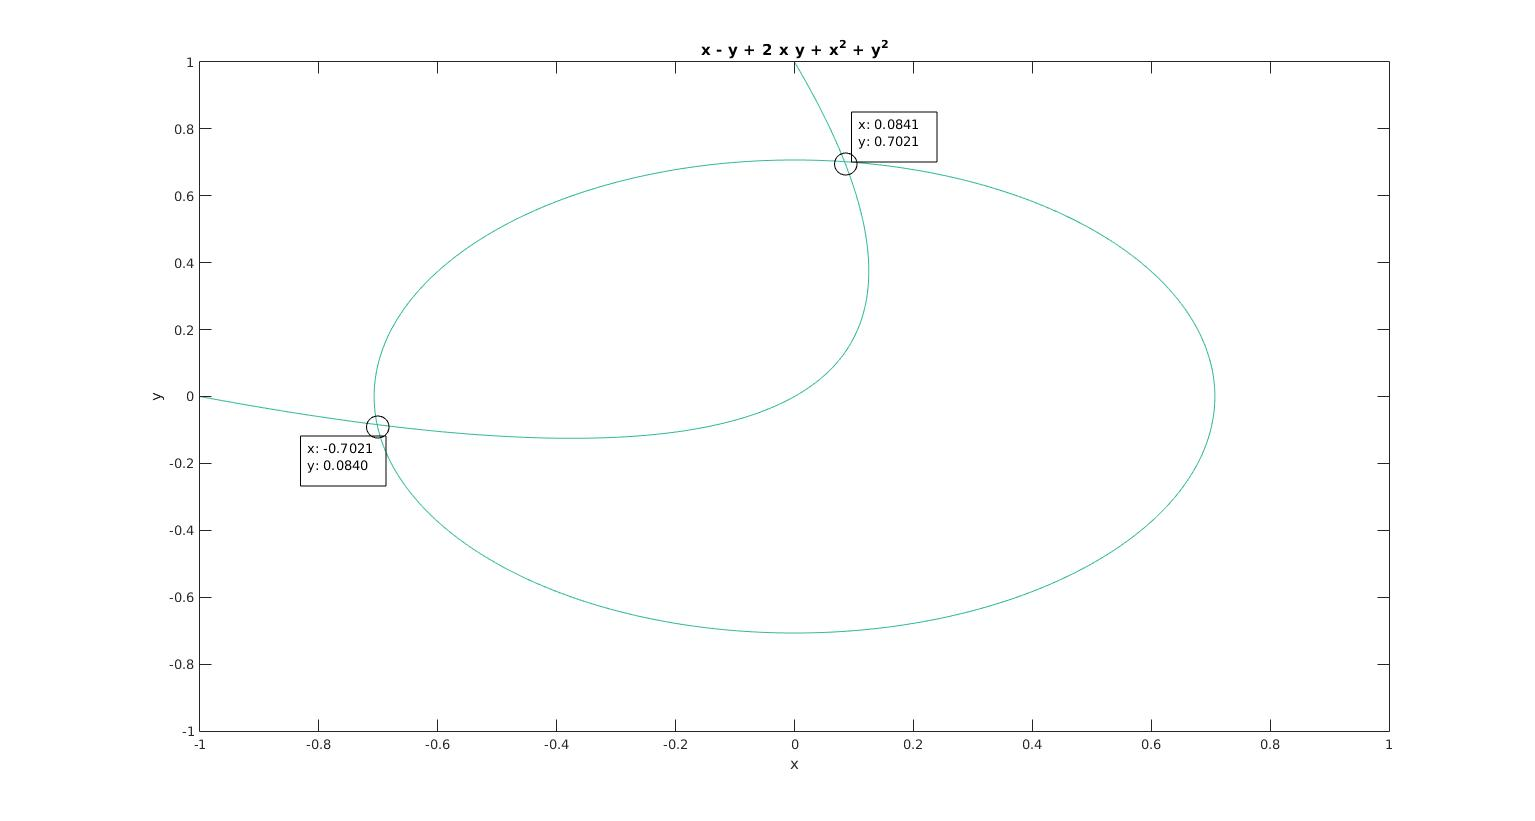
\includegraphics[width=5in]{p8-2.jpg}
\caption{graphing of the two functions}
\end{figure}
\section{Q9}
\subsection*{9(a)}
The linear equation would be based on \hyperref[https://en.wikipedia.org/wiki/Barycentric_coordinate_system]{Barycentric coordinate system} which says that each point in a triangle could be written by three Barycentric coordinates. The three barycentric coordinates will be set as $v$ in the linear equation.
\begin{equation*}
\begin{pmatrix}
x^{(i)} & x^{(j)} & x^{(k)} \\
y^{(i)} & y^{(j)} & y^{(k)} \\
1 & 1 & 1 
\end{pmatrix}
\begin{pmatrix}
v_0 \\
v_1 \\
v_2 
\end{pmatrix}
=
\begin{pmatrix}
x \\
y \\
1 
\end{pmatrix}
\end{equation*}
\subsection*{9(b)}
The algorithm is implemented in the function in \textit{interpolatePath.m}.\\
The Algorithm that is used to find the 3 paths are as following:
\begin{enumerate}
	\item find the path with the closet start point to the start point given. That path will be the first path($p_1$).
	\item calculate the distance of all points to the start point of $p_1$.
	\item if $p_1$ has $x > y$, pick two paths with the closet start point where their $x$ is also $> y$. Those two path become $p_2$ and $p_3$. 
	\item if $p_1$ has $x <= y$, pick two paths with the closet start point where their $x$ is also $<= y$. Those two path become $p_2$ and $p_3$. 
\end{enumerate}
To get the alpha, I used the linear equation in $9(a)$ and plugged in the values from $p_1$,$p_2$,$p_3$ and the starting point. Following is the equation used.
\begin{equation*}
\begin{pmatrix}
x^{p_1} & x^{p_2} & x^{p_3} \\
y^{p_1} & y^{p_2} & y^{p_3} \\
1 & 1 & 1 
\end{pmatrix}
\begin{pmatrix}
\alpha_1 \\
\alpha_2 \\
\alpha_3 \\ 
\end{pmatrix}
=
\begin{pmatrix}
startPoint_x \\
startPoint_y \\
1 
\end{pmatrix}
\end{equation*}
Currently, the time scale is 100. There is no particular reason for picking this time scale besides is a multiple of the time scale given(50).
\subsection*{9(c)}
The following is the plot of the interpolate path. The given paths are in yellow. The path with the starting point$(0.8, 1.8)$ is the path colored red. The path with the starting point $(2.2, 1.0)$ is the path colored greeen. the path with the starting point $(2.7, 1.4)$ is the path colored blue.
\begin{figure}[h]
\centering
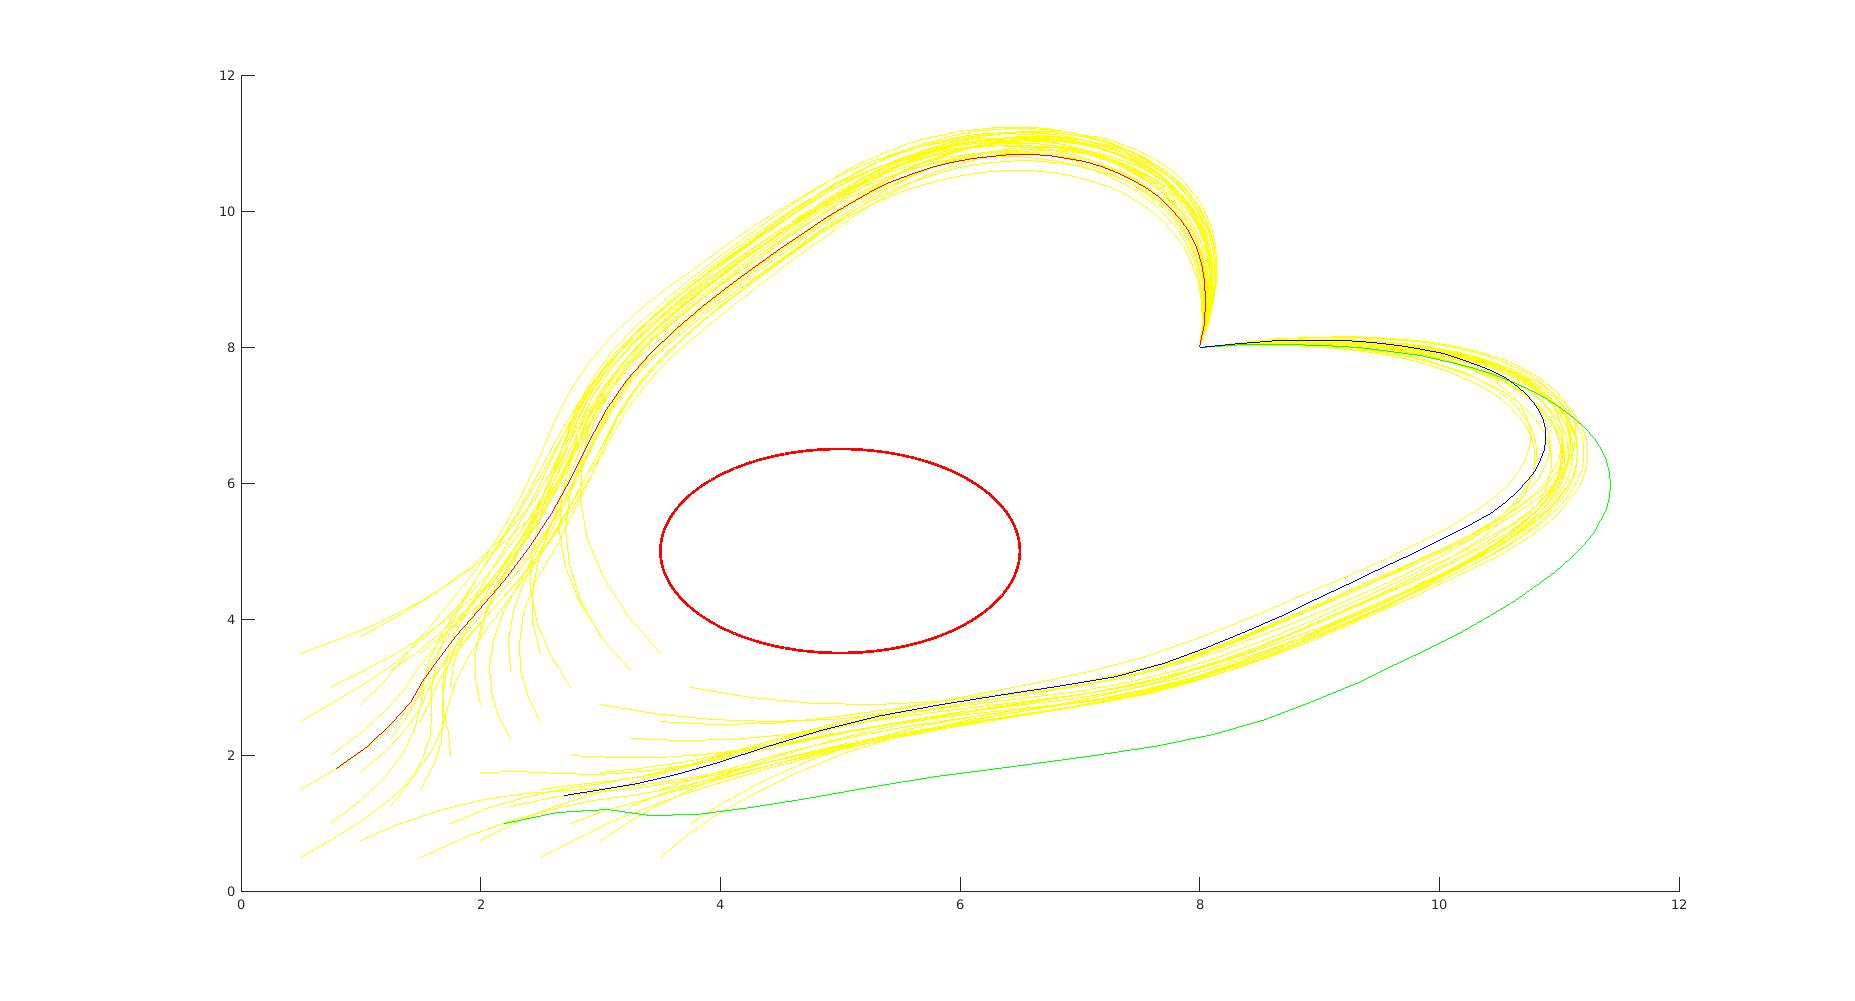
\includegraphics[width=6in]{p9.jpg}
\end{figure}\\
\subsection*{9(d)}
If you observe the graph, you will notice that certain interpolate path goes further out that the given paths. This would be a problem if there are more obstacles that are introduced near the path. One possible additiona to the algorithm is to recalculate the weights and interpolation path after a certain interval. Let say t is 100, we could recalculate all these values in 20 intervals. 



\end{document}